\documentclass{article}
\pagestyle{plain}
\usepackage{inputenc, amsmath, amssymb, amsfonts, url, caption, rotating, xcolor, enumitem, amsthm, hyperref, subcaption, braket, soul, scalerel, graphicx, hyphenat, float, cite}

%\usepackage[style=numeric-comp,backend=biber]{biblatex}
\DeclareRobustCommand{\comment}[1]{\textcolor{red}{#1}}

\usepackage[a4paper,top=2.5cm,bottom=2.5cm,left=2.5cm,right=2.5cm]{geometry}
\newcommand*\xbar[1]{%
  \hbox{%
    \vbox{%
      \hrule height 0.3pt % The actual bar
      \kern0.3ex%         % Distance between bar and symbol
      \hbox{%
        \kern-0.1em%      % Shortening on the left side
        \ensuremath{#1}%
        \kern-0.1em%      % Shortening on the right side
      }%
    }%
  }
}

\newcommand{\Avg}[1]{\mathbb{E}\left[#1\right]}
\newcommand{\Var}[1]{\text{Var}\left[#1\right]}
\newcommand{\covar}[1]{\text{Cov}\left[#1\right]}
\newcommand{\cv}[1]{\text{CV}_{#1}}
\newcommand{\avg}[1]{\langle#1\rangle}
\newcommand{\Th}{_\mathrm{th}}



\begin{document}

\begin{center}
  {\Large\textsc{Bachelor Thesis Summary}\par}\vfill % \par assicura la giusta spaziatura
  {\LARGE\bfseries Simulation of LiteBIRD Instrumental Noise \\ with the LBS Framework \par}\vfill 
  {\large Corso di Laurea in Fisica -- Università degli Studi di Milano\\
  Academic Year 2024--2025\par}
\end{center}

{\large
  \begin{tabular}{@{}l l@{}}
    \textbf{Candidate:}  & Giulia Giommoni \\ 
    \textbf{Supervisor:} & Prof. Maurizio Tomasi \\
  \end{tabular}
}



\section*{Scientific Context and Objectives}
LiteBIRD (LiteB-mode polarization and Inflation from cosmic background Radiation Detection) is a space mission aimed at detecting primordial B-mode polarization in the Cosmic Microwave Background (CMB). This would prove the existence of cosmic inflation by capturing signals from primordial gravitational waves. LiteBIRD targets both the recombination peak ($\ell \simeq 80$) and the reionization peak ($\ell \lesssim 10$). Access to these large angular scales is only possible from space, but measurements are highly sensitive to low-frequency correlated noise and long-term instrumental drifts.

The primary objective of this thesis is the modeling, implementation, and comparison of instrumental noise models, in particular white noise and correlated $1/f$ noise, with the LiteBIRD Simulation (LBS) framework. To support long-duration mission simulations, I introduce a block-wise processing architecture capable of handling large amounts of data with high memory efficiency.



\section*{Noise Modeling and TOD Management}
Instrumental noise is characterized by two components: 
\begin{itemize}
    \item White Noise: a stochastic process with a flat Power Spectral Density (PSD), $P(f) = \sigma^2$.
    \item 1/f Noise: a correlated component that exhibits low-frequency drifts, with a PSD following $P(f) \approx \sigma^2(f_{knee}/f)^\alpha$.
\end{itemize}

In these models, $\sigma^2$ represents the white noise level and $f_{knee}$ the knee frequency.

The detector output is stored as Time-Ordered Data (TOD), a 2D array ($N_{detectors} \times M_{samples}$). As $M$ grows linearly with observation time, full-mission TODs quickly exceed the memory capacity. In this thesis I implement a block-wise approach, splitting the TOD into finite-duration segments. This ensures memory efficiency, scalability, and enables parallelization.



\section*{Implementation: LBS vs. ducc0}
I developed two distinct functions to perform in-place noise addition, both based on pre-existing noise-generation functions. The first, \texttt{add\_lbsNoise}, is integrated into the LBS (LiteBIRD Simulation) framework, the official Python-based library of the collaboration. The second, \texttt{add\_OofaNoise}, utilizes the ducc0 (Distinctly Useful Code Collection) library, a high-performance C++ package designed for efficient astronomical data processing.

The two functions are implemented as follows:
\begin{itemize}
    \item \texttt{add\_lbsNoise}: utilizes the pre-existing \texttt{lbs.add\_noise} function, which relies on FFT-based stochastic generation. While it offers high spectral flexibility (arbitrary PSDs), it requires larger memory buffers and can introduce discontinuities at block boundaries.
    \item \texttt{add\_OofaNoise}: relies on the \texttt{ducc0.misc.OofaNoise} class, which employs recursive digital filtering. It provides intrinsic temporal continuity across blocks and a minimal, constant memory footprint, though it is constrained to a rigid $1/f^\alpha$ model.
\end{itemize}



\section*{Time and Frequency Domains Analysis}
First, I validated my code using short-term simulations for statistical confirmation of the models. In the time domain, $1/f$ noise correctly manifests as coherent, slow-varying waves. In the frequency domain, the estimated PSDs follow the theoretical trend: the high-frequency white noise plateau and the $f^{-\alpha}$ slope below the knee frequency.


\begin{figure}[htbp]
     \centering
     \begin{subfigure}[b]{0.4\textwidth}
         \centering
         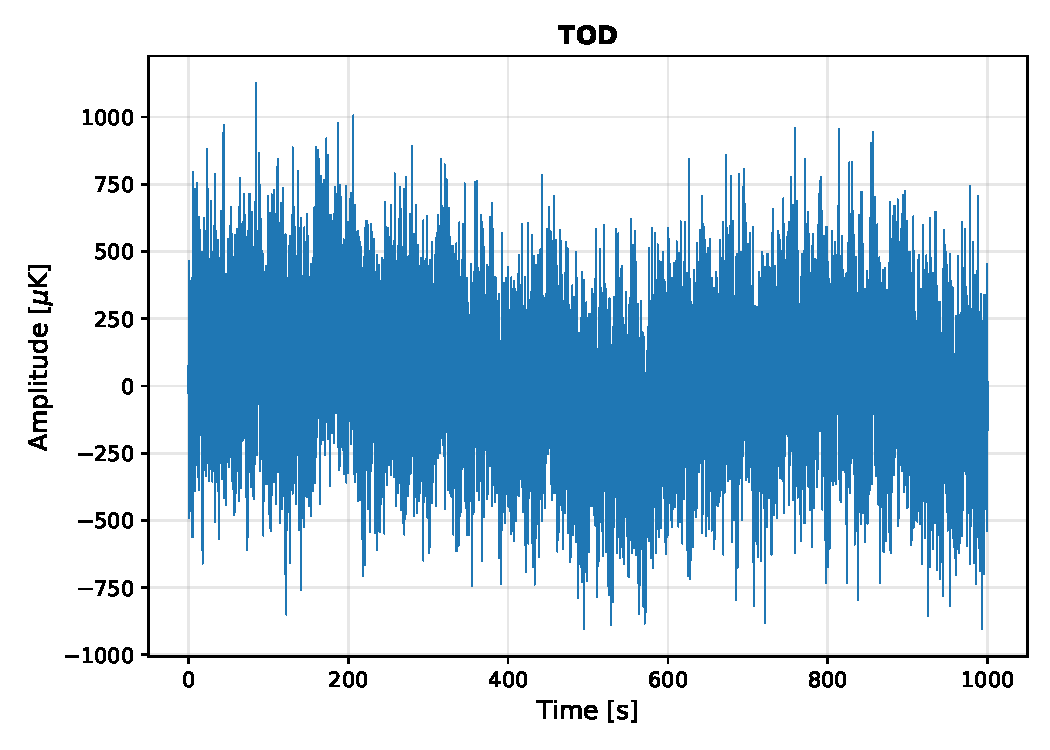
\includegraphics[width=\textwidth]{graph_tod.pdf}
         \label{fig:tod}
     \end{subfigure}
     \hspace{6mm} 
     \begin{subfigure}[b]{0.4\textwidth}
         \centering
         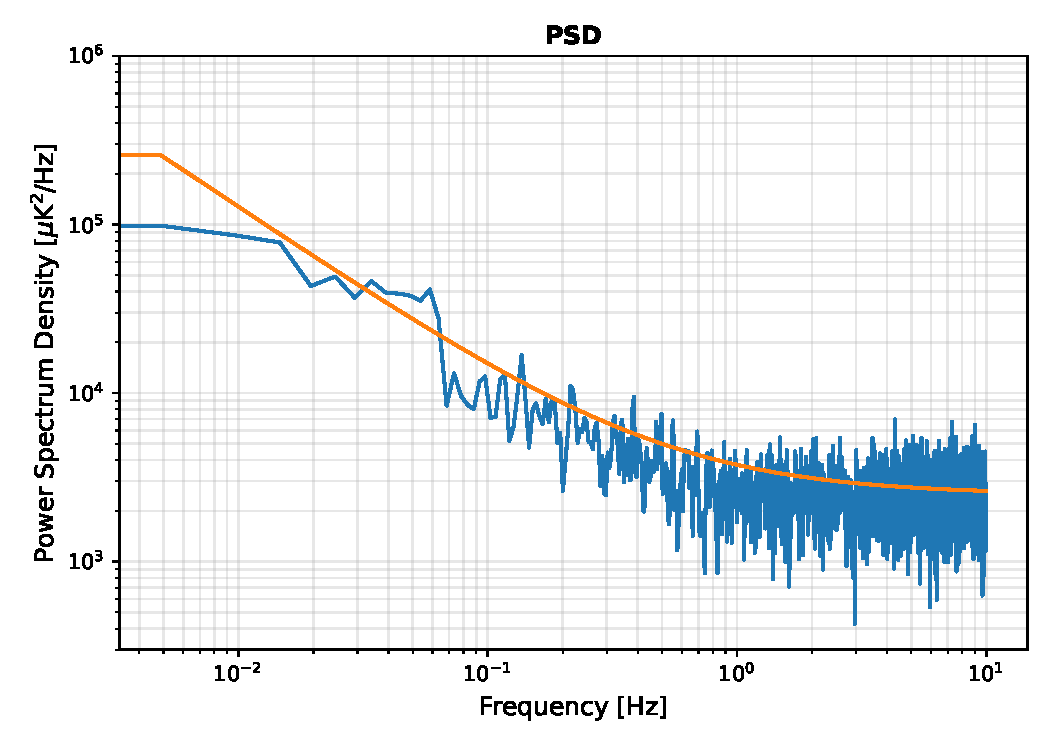
\includegraphics[width=\textwidth]{graph_psd.pdf}
         \label{fig:psd}
     \end{subfigure}
    \caption{Statistical validation of the noise models. Left: Time-Ordered Data (TOD) showing the characteristic low-frequency drifts of $1/f$ noise over a 1000s simulation. Right: Power Spectral Density (PSD) estimate showing the transition from the $f^{-\alpha}$ correlated regime to the white-noise plateau.}     \label{fig:noise_comparison}
\end{figure}



\section*{Map-Making and Harmonic Analysis}
To assess the spatial impact of noise, I conducted long-term simulations (up to one year) using a map-making pipeline, which uses JIT functions for optimization. 

The resulting maps show typical stripping patterns. These are the result of temporal $1/f$ correlations along the telescope's scanning paths. I confirmed that the scanning strategy’s redundancy helps reduce these drifts through the crossing of different scans. This effect is particularly evident in regions with high hit-counts where the noise pattern appears more attenuated.

\begin{figure}[htbp]
     \centering
     \begin{subfigure}[b]{0.4\textwidth}
         \centering
         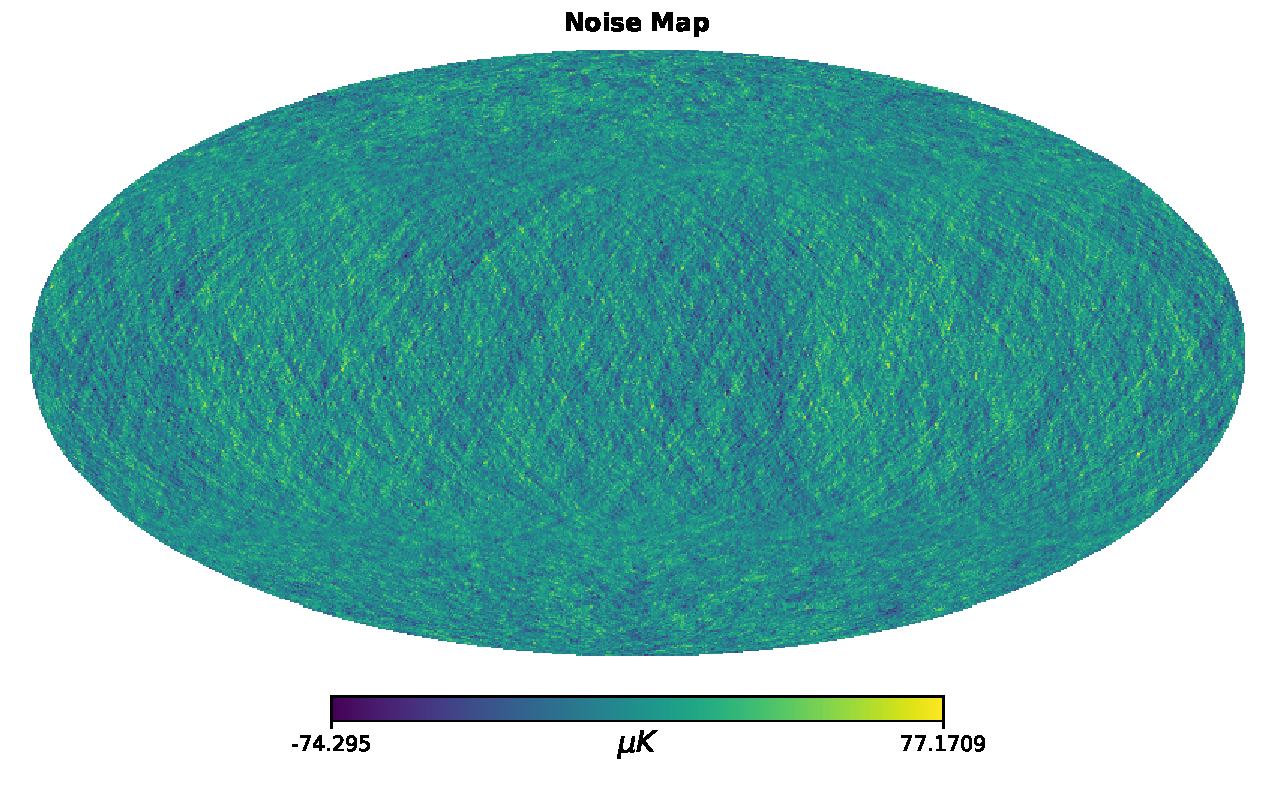
\includegraphics[width=\textwidth]{map.pdf}
         \label{fig:tod}
     \end{subfigure}
     \hspace{6mm} 
     \begin{subfigure}[b]{0.4\textwidth}
         \centering
         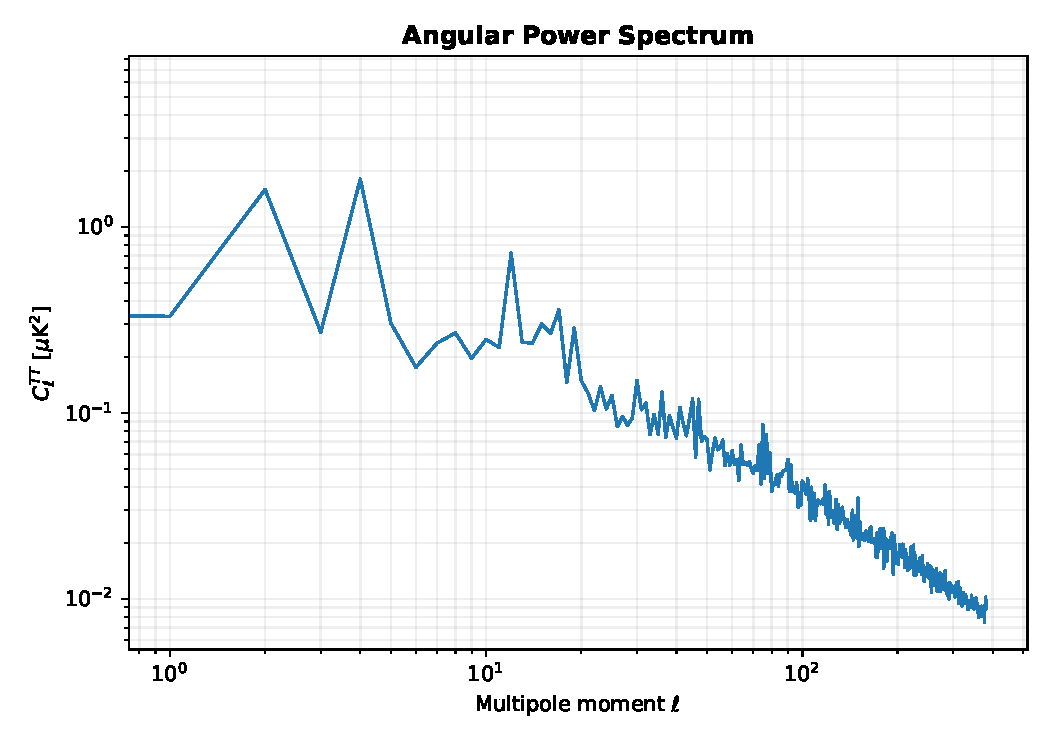
\includegraphics[width=\textwidth]{graph_psTT.pdf}
         \label{fig:psd}
     \end{subfigure}
    \caption{Spatial manifestation of instrumental noise. Left: HEALPix noise-only map generated from a one-year simulation, where the striation patterns reveal the projection of temporal correlations along the scanning strategy. Right: Angular power spectrum $C_\ell^{TT}$ derived from the map, assuming no correction for $1/f$ noise in the map-making. The steep rise at low multipoles highlights the dominance of correlated noise on large angular scales. This low-multipole noise is usually cleaned at the map-level in data reduction pipelines; here we preserved it to highlight its potential impact on the power spectrum if not properly treated.}     \label{fig:noise_comparison}
\end{figure}

Finally, I characterized the noise in the harmonic domain ($C_\ell^{TT}$). Both models show a consistent descending slope at low multipoles ($\ell$), representing the large-scale spatial correlations induced by $1/f$ noise. Due to the high $f_{knee}$ value used in the tests, this correlated component dominates the spectrum, masking the white noise plateau.



\section*{Conclusions} 
In my thesis, I demonstrated that both implemented functions produce valid results and correctly reproduce the expected noise physics. While \texttt{add\_lbsNoise} uses a standard, verified FFT-based method widely used and serves as a versatile tool for non-standard spectra, \texttt{add\_OofaNoise} offers a more robust and memory-efficient solution for large-scale mission simulations. Most importantly, the implementation of the block-wise processing framework proves to be a computational necessity, enabling the simulation of realistic TOD durations.
\end{document}
